\section{The Model Used For this project : ResNet50V2}

\begin{flushleft}

In this project it was used as starting point the ResNet50V2 CNN network (available on Tensorflow library). The choice of the use of such network is due to some mainly two reasons :
\begin{itemize}
    \item The ResNet50 (V1) Network contrary to what is said in [reference paper 3] was performing poorly in the dataset used for our training if fine tuned
    \item The ResNet50 (V1) Netwoork was able to learn something on the dataset used only if it was trained from scratch (no fine tuning) on the entire dataset but, due to low hardware performances available the training on the entire dataset was carried out only for one epoch before running out of both RAM and GPU RAM memories.
\end{itemize}
\begin{center}
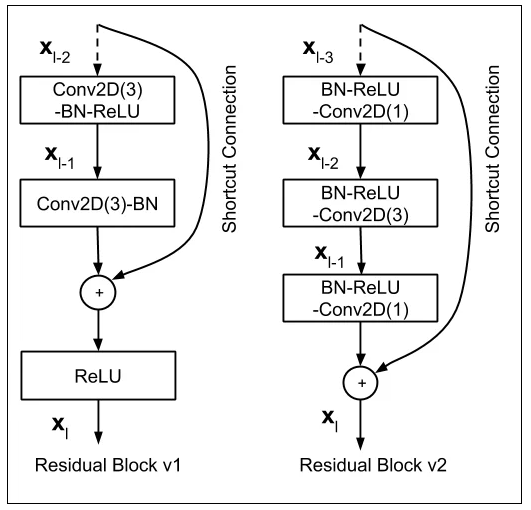
\includegraphics[scale = 0.35]{images/RenetVersus.PNG}    
\end{center}
So, for the reason explained above it was chosen the ResNet50V2 and it was fine tuned by removing its fully connected layers and replaced them with other two. To be precise:
\begin{itemize}
    \item A layer with 1024 neurons with Relu activation function.
    \item A layer with 2 neurons with Sigmoid activation function.
\end{itemize}
\begin{center}
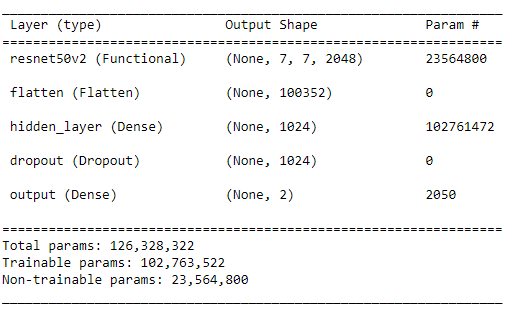
\includegraphics[scale = 0.70]{images/ModelUsed.PNG}    
\end{center}

In addition to that, to avoid over fitting issues some regularization techniques were applied. The most important ones are :
\begin{itemize}
    \item Early Stopping on the validation loss
    \item Data Augmentation on the batch items
    \item Validation on hyper parameters of the network 
\end{itemize}




\end{flushleft}